\newpage
\section{Forsyth-Edwards Notation}
Forsyth-Edwards Notation (FEN) is a way to describe the current state of a chessboard using only ASCII characters. Based on a system first developed by David Forsyth, a Scottish journalist. Well knowns chess engines, such as the open spurce Stockfish use the FEN notation as an input to determine the best moves.\\

The notation consists of 6 elements in the following order:\cite{wiki:FEN}
\begin{enumerate}
    \item Piece placement. As shown in figure \ref{fig:03:FEN_workings}. Each rank is comprised into a string  where each piece has a letter corresponding to it. It is ordered rank 8 to 1 and from "a" to "h", each rank being sepparated by a "/". It follows the Standard Algebraic Notation (SAN) for the pieces, where each piece gets its name from the first pronounced letter of their english names. If a squere is empty it is notated by a number from 1-8, where the number represent the number of open spaces in a row. upper-case letters indicate white, while black is represented by lower-case. 
    \item Indication of active player, "w" for white and "b" for black.
    \item Indicated the types of casteling that is available, "KQkq" means that all casteling both to queen and king side is possible. "Kq" means that white can castle to the king-side, while black has the option to castle to the queen-side.
    \item En passant target square in algebraic form, in the event of a pawn moves two quares, en pessant will be the square behind. if there is no pawn in possition to do an en passant move, it is simply denoted by "-".
    \item Halfmove clock. A counter that resets uppon pawn capture, it determines wether or not a draw can be claimed under the fifty-move rule.
    \item Fullmove number. Starts at 1 and increments every time black moves.
\end{enumerate}

\begin{figure}[H]
    \centering
    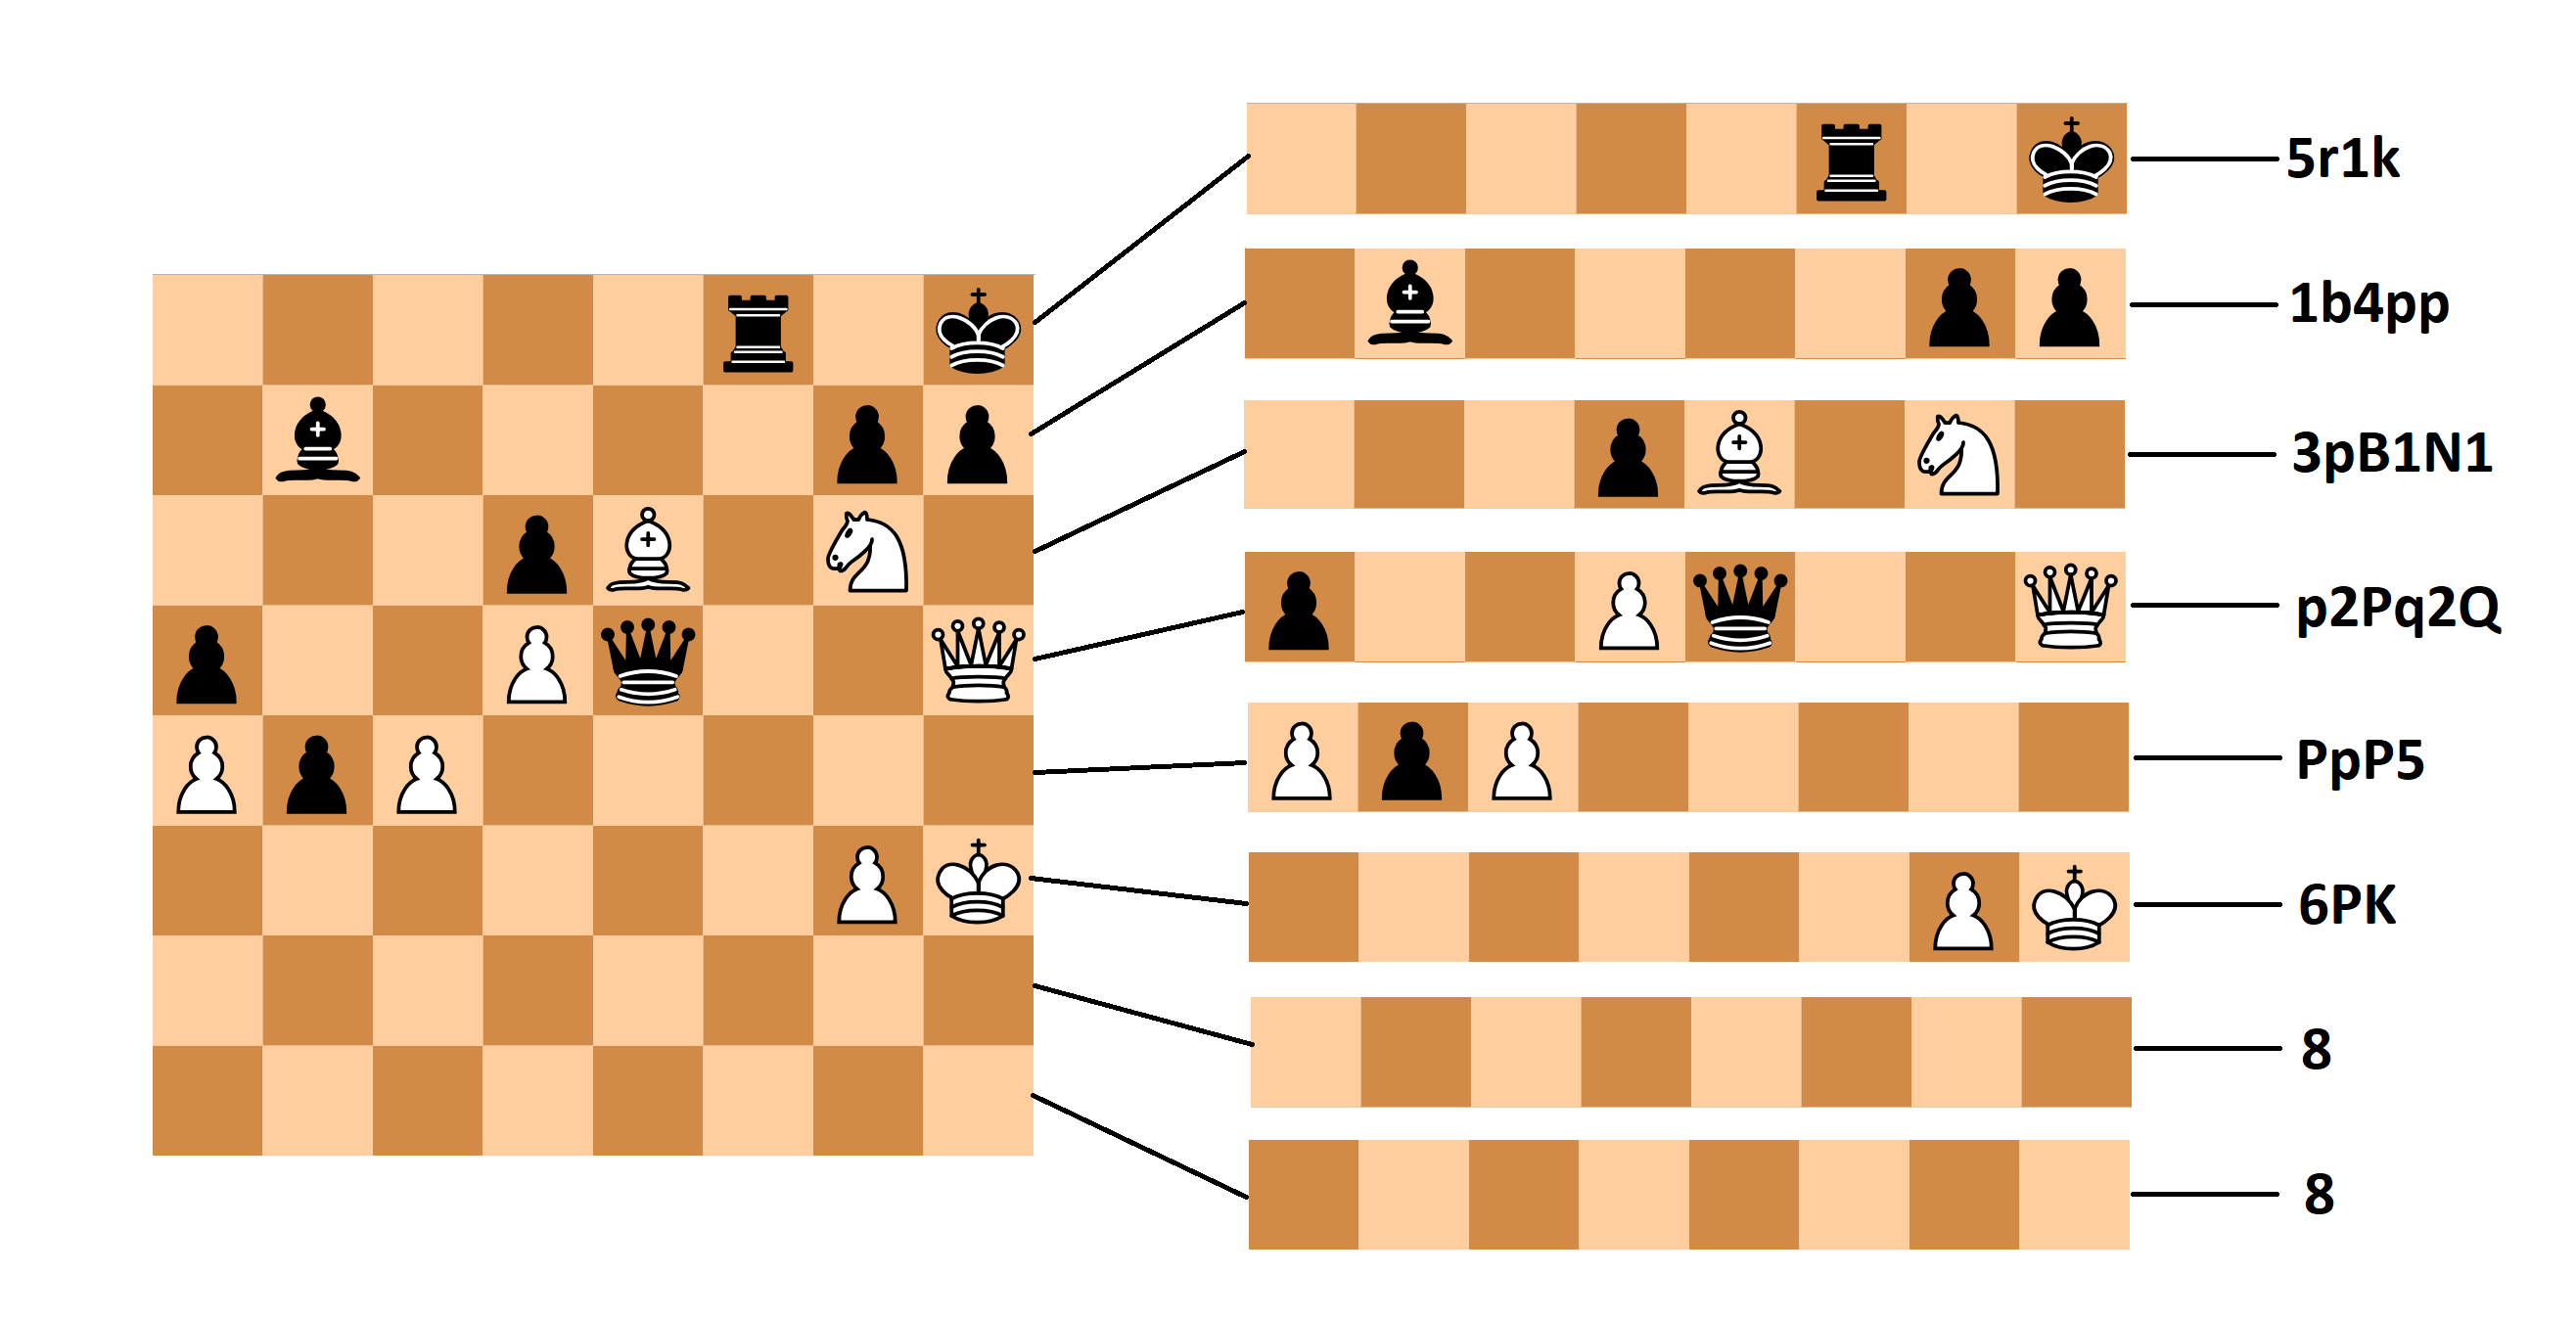
\includegraphics[width=\textwidth]{03_Theory/figures/FEN_explain.png}
    \caption{How the FEN piece placement works}
    \label{fig:03:FEN_workings}
\end{figure}